\subsubsection{Ý tưởng}
Bubble Sort là thuật toán sắp xếp so sánh liên tiếp các cặp phần tử liền kề trong mảng và hoán đổi nếu chúng không theo đúng thứ tự. Quá trình này được lặp lại cho đến khi mảng được sắp xếp. Với mỗi lần lặp, các phần tử sẽ được đưa về đúng vị trí của nó, giống như các bong bóng nổi lên từ dưới đáy nước. \cite{black2009}
\subsubsection{Mã giả}

\begin{algorithm}[H]
\caption{BubbleSort}
\begin{algorithmic}[1]
\Procedure{BubbleSort}{$arr, n$}
    \State \textbf{Input:} Mảng $arr$ gồm $n$ phần tử
    \State \textbf{Output:} Mảng $arr$ được sắp xếp
    
    \For {$i \gets 0 $ \textbf{to} $n$}
        \For {$j \gets 0$ \textbf{to} $n - i - 1$} 
            \If{$arr[j] > arr[j+1]$}
                \State \textbf{swap} $arr[j]$ \textbf{and} $arr[j+1]$
            \EndIf
        \EndFor
    \EndFor
\EndProcedure
\end{algorithmic}
\end{algorithm}

\subsubsection{Ví dụ}

Dưới đây là các bước chạy tay của thuật toán \textit{Bubble Sort} với mảng $[42, 17, 93, 58, 21, 76, 34]$:
\begin{figure}[H]
    \centering
    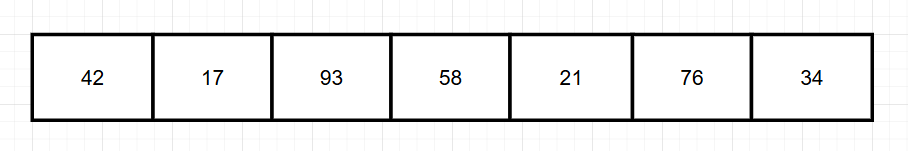
\includegraphics[width=0.75\linewidth]{img/bubble_sort/1.png}
\end{figure}

Trong mỗi lần lặp ta sẽ tiến hành so sánh các phần tử liền kề và hoán đổi chúng nếu chúng không theo thứ tự và cứ tiếp tục như cho đến hết mảng.
\newpage
\begin{enumerate}
    \item Lần lặp thứ nhất
    \begin{figure}[H]
        \centering
        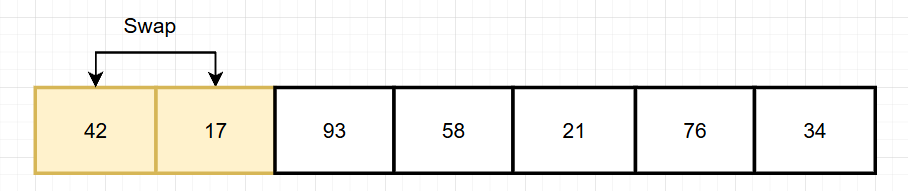
\includegraphics[width=0.75\linewidth]{img/bubble_sort/2.png}
        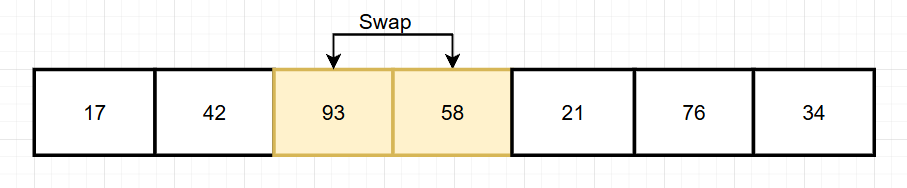
\includegraphics[width=0.75\linewidth]{img/bubble_sort/3.png}
        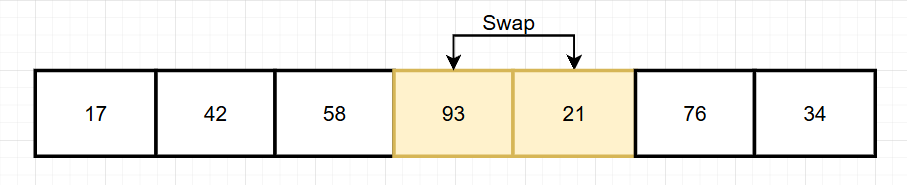
\includegraphics[width=0.75\linewidth]{img/bubble_sort/4.png}
        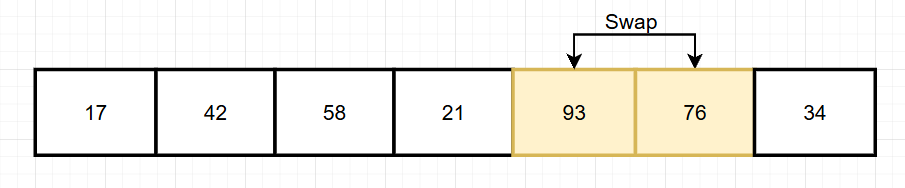
\includegraphics[width=0.75\linewidth]{img/bubble_sort/5.png}
        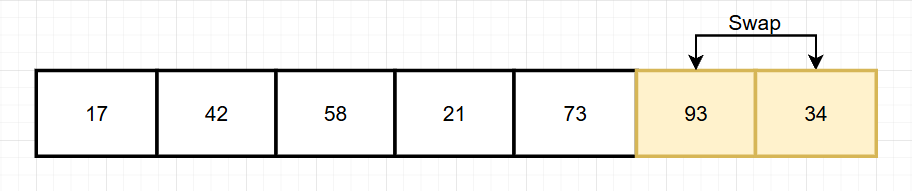
\includegraphics[width=0.75\linewidth]{img/bubble_sort/6.png}
        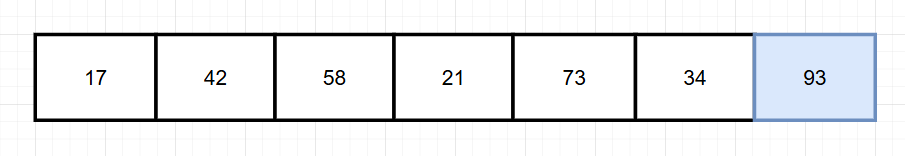
\includegraphics[width=0.75\linewidth]{img/bubble_sort/7.png}
    \end{figure}

    \begin{figure}[H]
        \centering
        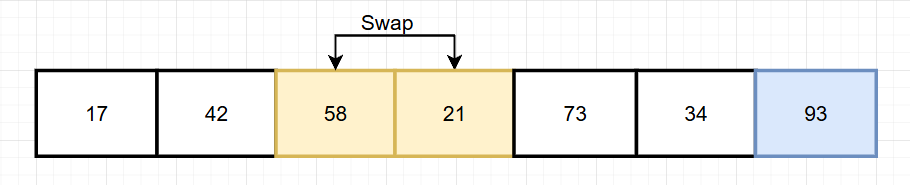
\includegraphics[width=0.75\linewidth]{img/bubble_sort/8.png}
        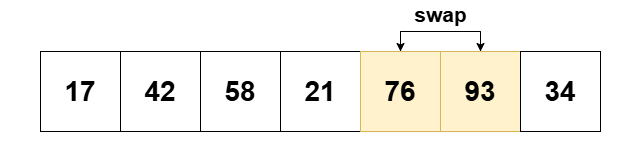
\includegraphics[width=0.75\linewidth]{img/bubble_sort/9.png}
        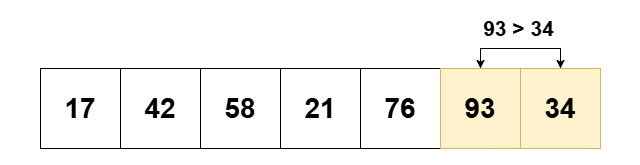
\includegraphics[width=0.75\linewidth]{img/bubble_sort/10.png}
        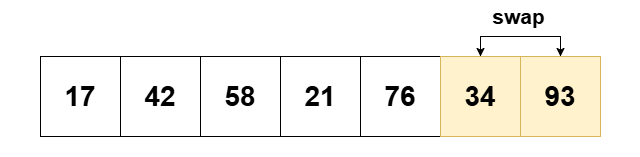
\includegraphics[width=0.75\linewidth]{img/bubble_sort/11.png}
        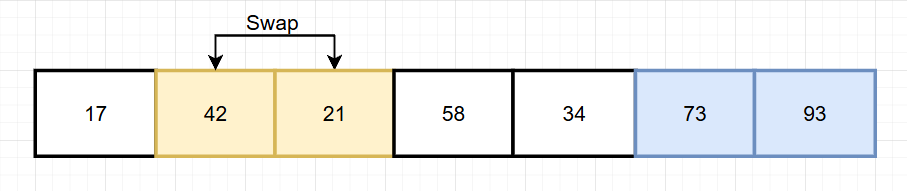
\includegraphics[width=0.75\linewidth]{img/bubble_sort/12.png}
    \end{figure}

    \item Lần lặp thứ hai
    \begin{figure}[H]
        \centering
        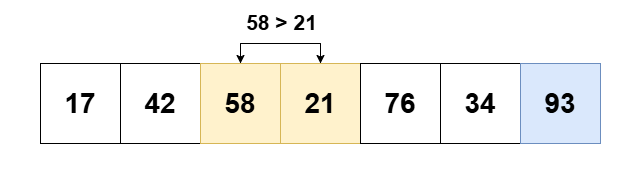
\includegraphics[width=0.75\linewidth]{img/bubble_sort/13.png}
       
    \end{figure}

    \begin{figure}[H]
        \centering
        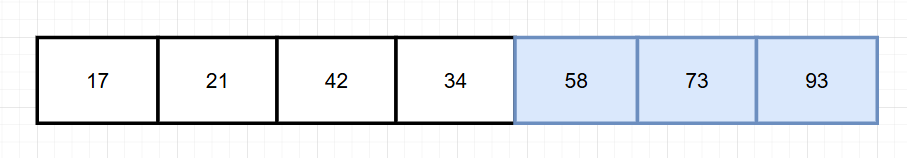
\includegraphics[width=0.75\linewidth]{img/bubble_sort/14.png} 
        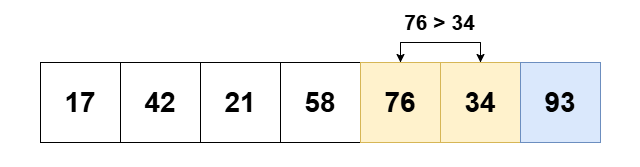
\includegraphics[width=0.75\linewidth]{img/bubble_sort/15.png}
        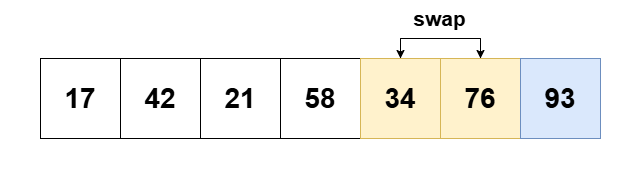
\includegraphics[width=0.75\linewidth]{img/bubble_sort/16.png}
        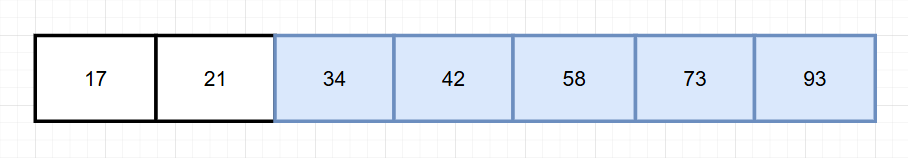
\includegraphics[width=0.75\linewidth]{img/bubble_sort/17.png}        
    \end{figure}

    \item Lần lặp thứ ba
    \begin{figure}[H]
        \centering
        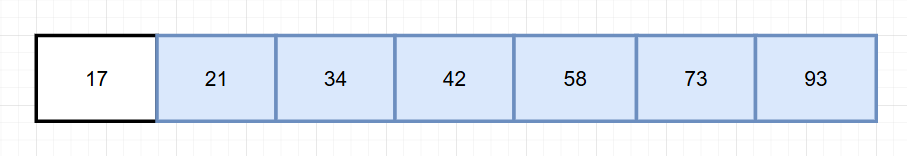
\includegraphics[width=0.75\linewidth]{img/bubble_sort/18.png}
        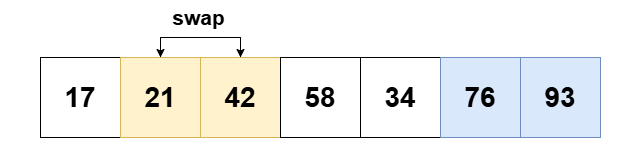
\includegraphics[width=0.75\linewidth]{img/bubble_sort/19.png}
    \end{figure}

    \begin{figure}[H]
        \centering
        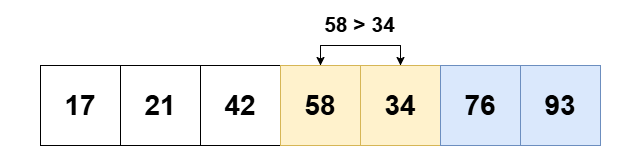
\includegraphics[width=0.75\linewidth]{img/bubble_sort/20.png}
        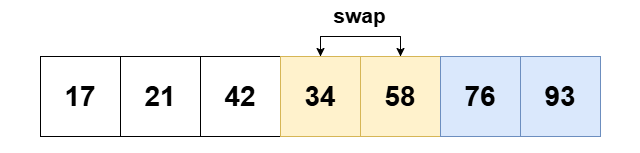
\includegraphics[width=0.75\linewidth]{img/bubble_sort/21.png}
        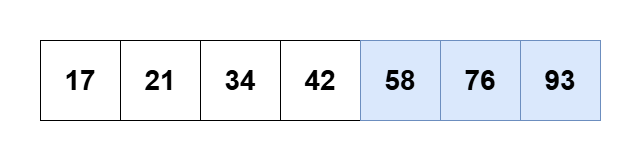
\includegraphics[width=0.75\linewidth]{img/bubble_sort/22.png}
    \end{figure}

    \item Lần lặp thứ tư
    \begin{figure}[H]
        \centering
        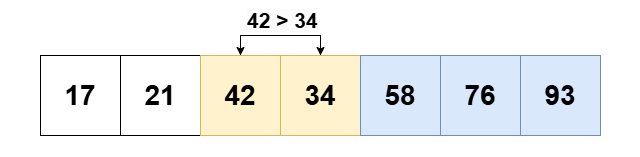
\includegraphics[width=0.75\linewidth]{img/bubble_sort/23.png}
        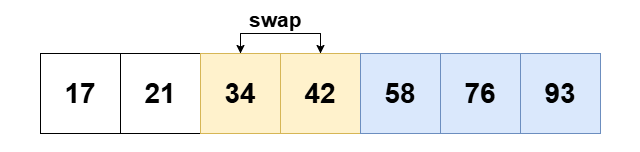
\includegraphics[width=0.75\linewidth]{img/bubble_sort/24.png}
        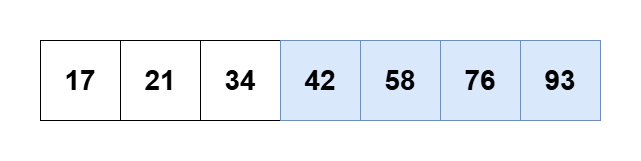
\includegraphics[width=0.75\linewidth]{img/bubble_sort/25.png}
    \end{figure}
    \newpage
    \item Lần lặp thứ năm
    \begin{figure}[H]
        \centering
        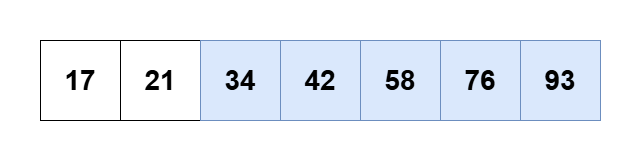
\includegraphics[width=0.75\linewidth]{img/bubble_sort/26.png}
    \end{figure}

    \item Lần lặp thứ sáu
    \begin{figure}[H]
        \centering
        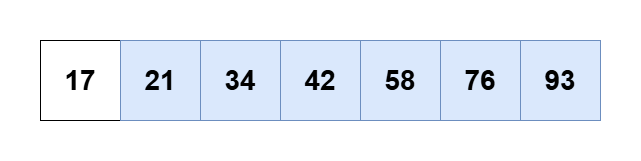
\includegraphics[width=0.75\linewidth]{img/bubble_sort/27.png}
    \end{figure}

    \item Lần lặp thứ bảy
    \begin{figure}[H]
        \centering
        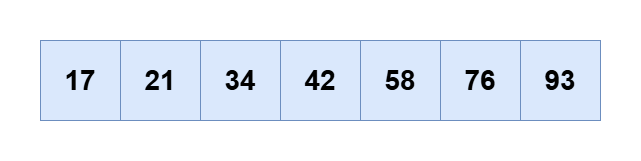
\includegraphics[width=0.75\linewidth]{img/bubble_sort/28.png}
    \end{figure}

    \item Cuối cùng ta thu được mảng được sắp xếp
    \begin{figure}[H]
        \centering
        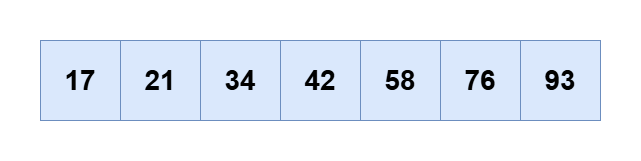
\includegraphics[width=0.75\linewidth]{img/bubble_sort/28.png}
    \end{figure}
\end{enumerate}
\newpage
\subsubsection{Độ phức tạp}

\begin{itemize}
    \item[\textbf{--}]\textbf{Thời gian:} Vì mỗi lần lặp ta đều phải duyệt qua toàn bộ mảng nên cả 3 trường hợp đều có độ phức tạp là:
        \begin{itemize}
            \item[\textbullet]\textbf{Best case}: $\mathcal{O}(n^2)$
            \item[\textbullet]\textbf{Average case}:  $\mathcal{O}(n^2)$
            \item[\textbullet]\textbf{Worst case}:  $\mathcal{O}(n^2)$
        \end{itemize}
    \item[\textbf{--}]\textbf{Không gian:}  $\mathcal{O}(1)$, vì không cần thêm bộ nhớ phụ trong quá trình sắp xếp.
    \item[\textbf{--}]\textbf{Tính ổn định:} \textit{Bubble sort} là thuật toán ổn định nghĩa là nó không thay đổi vị trí của các phần tử bằng nhau trong quá trình sắp xếp.
\end{itemize}